\chapter{Sviluppo e implementazione}
\label{chap:sviluppo-implementazione}

\section{Organizzazione e ciclo di sviluppo}
\label{sec:organizzazione-ciclo-sviluppo}
\noindent L'implementazione del modulo relativo alle note spesa si è basata su una fase preliminare di studio e analisi della codebase aziendale preesistente. Per garantire la piena coerenza con gli standard di Ergon, il lavoro è iniziato esaminando l'architettura dei file e la struttura dei servizi di rete già in uso. Contestualmente, è stata analizzata la struttura delle tabelle create nel database aziendale ospitato su un server di test, per comprendere le relazioni tra le entità e i vincoli dei dati che l'applicazione mobile avrebbe dovuto gestire.\\
Una volta acquisita la conoscenza necessaria, lo sviluppo vero e proprio ha seguito un approccio incrementale, partendo dall'infrastruttura di \textit{backend}. In primo luogo è stata modellata la classe di dominio per mappare l'entità principale del database remoto, ovvero \texttt{SpesaDettaglio}, per poi passare alla realizzazione dei nuovi \gls{endpointrestg} all'interno del controller dedicato denominato \texttt{NoteSpesaController}, prendendo ispirazione dai servizi già esistenti. Una peculiarità architetturale adottata nello sviluppo di questi web services è stata l'utilizzo quasi esclusivo di metodi HTTP POST, impiegati anche per le operazioni di recupero dati. Questa scelta è stata dettata dalla necessità di garantire sicurezza e coerenza progettuale, permettendo di incapsulare e trasmettere in modo sicuro le credenziali di autenticazione e i parametri di ricerca all'interno del corpo della richiesta, mantenendo così un'interfaccia omogenea con il resto dell'infrastruttura. \\
Lo sviluppo si è poi concentrato sul \textit{frontend} mobile, dove il codice è stato strutturato seguendo rigorosamente il pattern \gls{mvvm}, procedendo con la creazione dei modelli per la gestione dei dati sul dispositivo, come \texttt{SpesaDettaglio}, \texttt{SpesaTipologia} e \texttt{SpesaTipoPagamento}, lo sviluppo delle \textit{View} per l'interfaccia utente, tra cui \texttt{NoteSpesaView}, \texttt{DettaglioMeseView} e \texttt{AddNotaSpesaView}, e l'implementazione dei rispettivi \textit{ViewModel} per la gestione della logica di presentazione e dell'interazione con i servizi di rete.\\
Infine, il ciclo di sviluppo è terminato con una fase di iterazione e perfezionamento continuo, analizzando l'applicazione nel suo insieme e testando i flussi di lavoro sia personalmente che in collaborazione con il tutor aziendale. 


\section{Livello di presentazione}
\label{sec:implementazione-presentazione}
\noindent Al fine di garantire una netta separazione tra la componente grafica visiva e la logica di controllo sottostante, le interfacce grafiche sono state implementate in modo dichiarativo nei file \gls{xamlg}, riducendo al minimo indispensabile il codice scritto nei rispettivi \textit{code-behind}, i quali si limitano a gestire l'inizializzazione dei componenti visivi nativi. Il collegamento tra la rappresentazione grafica e la logica di business è stato realizzato associando le istanze dei \textit{ViewModel} al \texttt{BindingContext} di ciascuna \textit{View}.\\
I tre componenti principali del \textit{frontend} mobile in cui la visualizzazione, il flusso e la manipolazione dei dati poggiano interamente sui meccanismi di \textit{Data Binding} sono:
\begin{itemize}
    \item \texttt{NoteSpesaView}, che funge da schermata principale per la visualizzazione della lista dei resoconti mensili delle note spesa filtrati per anno;
    \item \texttt{DettaglioMeseView}, che mostra l'elenco delle singole note spesa per un mese selezionato;
    \item \texttt{AddNotaSpesaView}, che consente sia l'inserimento che la modifica di una nota spesa.
\end{itemize} 
\noindent All'interno delle schermate destinate alla visualizzazione di elenchi strutturati, come \texttt{NoteSpesaView} per i resoconti mensili e \texttt{DettaglioMeseView} per le singole note spesa, la gestione dinamica dei record sfrutta le proprietà della classe \texttt{ObservableCollection}. Questa collezione specializzata notifica in autonomia all'interfaccia utente qualsiasi modifica apportata agli elementi in memoria (come l'aggiunta, la modifica o la rimozione di una nota spesa), aggiornando i controlli grafici in tempo reale senza necessità di forzare o programmare un rinfresco manuale della pagina.\\
Per quanto riguarda la gestione dell'interattività e degli input, qualsiasi operazione eseguita dall'utente sui controlli grafici è stata orchestrata mediante l'astrazione dei comandi, con l'interfaccia \texttt{ICommand}. L'implementazione pratica di questa logica ha previsto l'adozione della libreria ufficiale di Microsoft \texttt{CommunityToolkit.Mvvm} (\cite{site:community-toolkit-mvvm}), la quale permette di semplificare la definizione di proprietà osservabili e comandi reattivi. Nella \texttt{AddNotaSpesaView}, ad esempio, la selezione di un cliente, l'apertura del selettore della tipologia di spesa o la pressione del pulsante per allegare lo scontrino non intercettano eventi grafici diretti, ma innescano l'esecuzione di specifici comandi esposti dal rispettivo \textit{ViewModel}. Questo approccio centralizza la logica di business all'interno del \textit{ViewModel}, il quale assume la responsabilità di validare asincronamente i dati inseriti nei form, invocare i servizi di persistenza locale e coordinare la navigazione tra le pagine. L'isolamento così ottenuto assicura che il livello di presentazione rimanga del tutto agnostico rispetto alla provenienza e alla destinazione dei dati, elevando la manutenibilità globale del software e agevolando eventuali operazioni di refactoring estetico della \gls{ui}.

\subsection*{Componenti riutilizzabili: GenericPopupView}
\noindent Una scelta progettuale volta a massimizzare il riutilizzo del codice e a mantenere la coerenza visiva dell'interfaccia utente ha riguardato la gestione delle finestre di dialogo modali. Invece di utilizzare gli alert predefiniti dei sistemi operativi o di implementare schermate di notifica e di conferma specifiche per ogni singola funzionalità, è stato codificato un componente grafico generico e altamente configurabile denominato \texttt{GenericPopupView}, di cui se ne mostrano degli esempi nella figura \ref{fig:popup}.\\
Questo pop-up specializzato estende le capacità di visualizzazione dell'applicazione offrendo un'interfaccia parametrica. In fase di istanziazione, il componente riceve dinamicamente una serie di argomenti che ne determinano la veste grafica e il comportamento: il titolo dell'operazione, il messaggio informativo, l'icona tematica (come gli indicatori di avviso, errore o funzionamento offline), il colore e i testi associati ai pulsanti di interazione. Il collegamento con la logica di business asincrona orchestrata dai \textit{ViewModel} viene stabilito esponendo un meccanismo di sincronizzazione basato sulla classe \texttt{TaskCompletionSource}. Ciò consente al flusso esecutivo chiamante di attendere in modo non bloccante la scelta dell'utente, intercettando il valore booleano restituito alla chiusura della finestra modale.\\
L'adozione di questa architettura risponde direttamente al principio dello sviluppo software \gls{dryg}, riducendo a zero la duplicazione di codice grafico per le interazioni modali. Centralizzando la struttura in un'unica vista generica, qualsiasi futuro intervento di refactoring estetico, ottimizzazione del layout o modifica del comportamento dei pop-up si propaga istantaneamente a tutte le funzionalità del modulo, innalzando notevolmente il livello di manutenibilità del \textit{frontend} mobile.
\begin{figure}[H]
    \centering
    \begin{tabular}{ccc}
        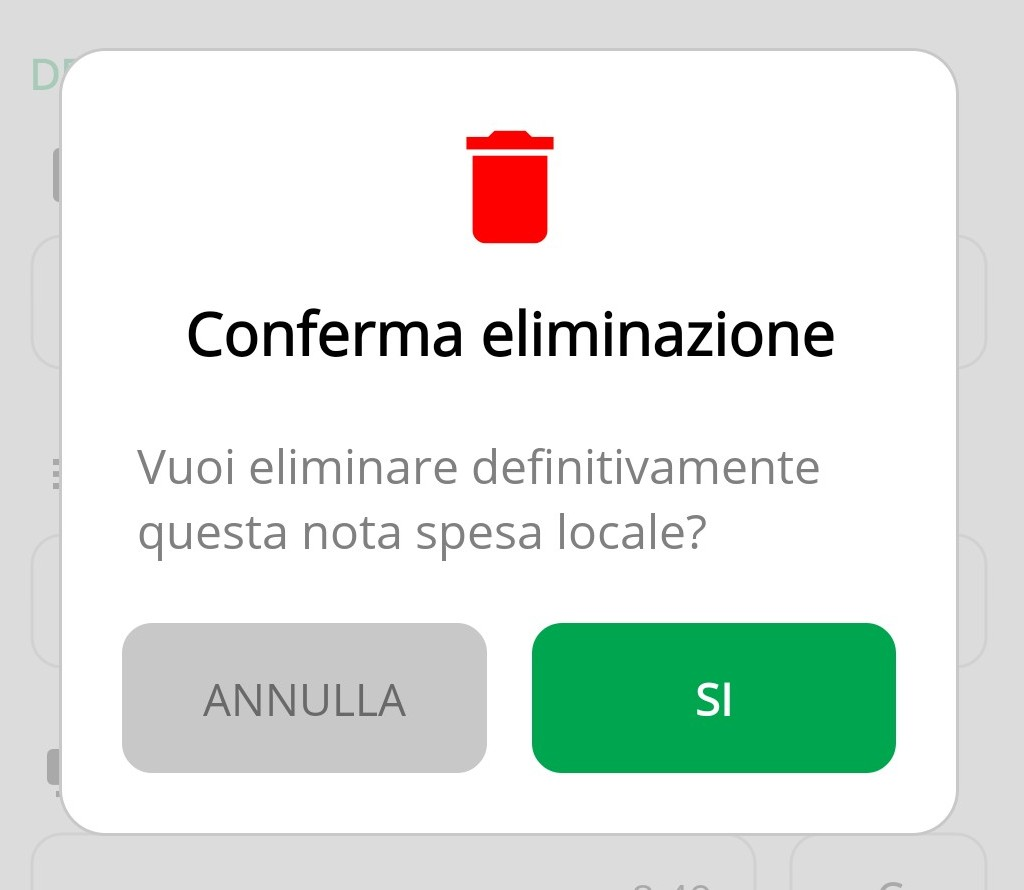
\includegraphics[width=0.29\textwidth]{img/screen/pp_conferma_eliminazione.jpg} &
        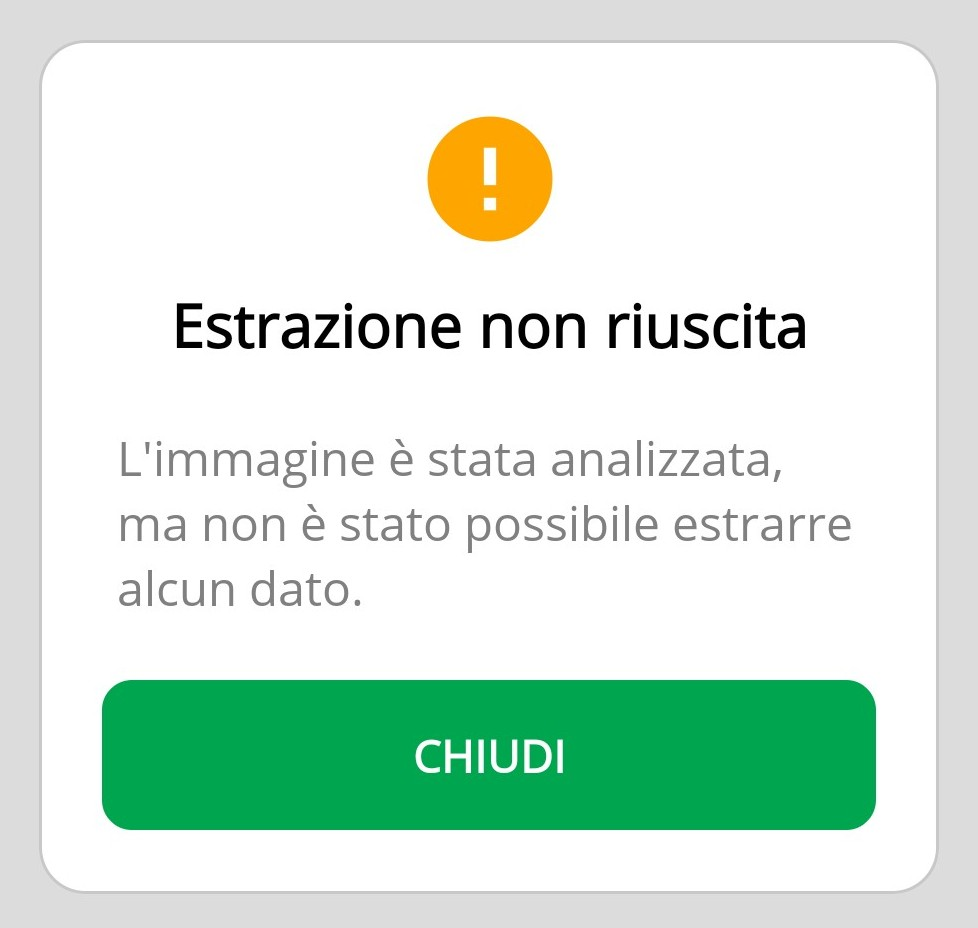
\includegraphics[width=0.29\textwidth]{img/screen/pp_estrazione.jpg} &
        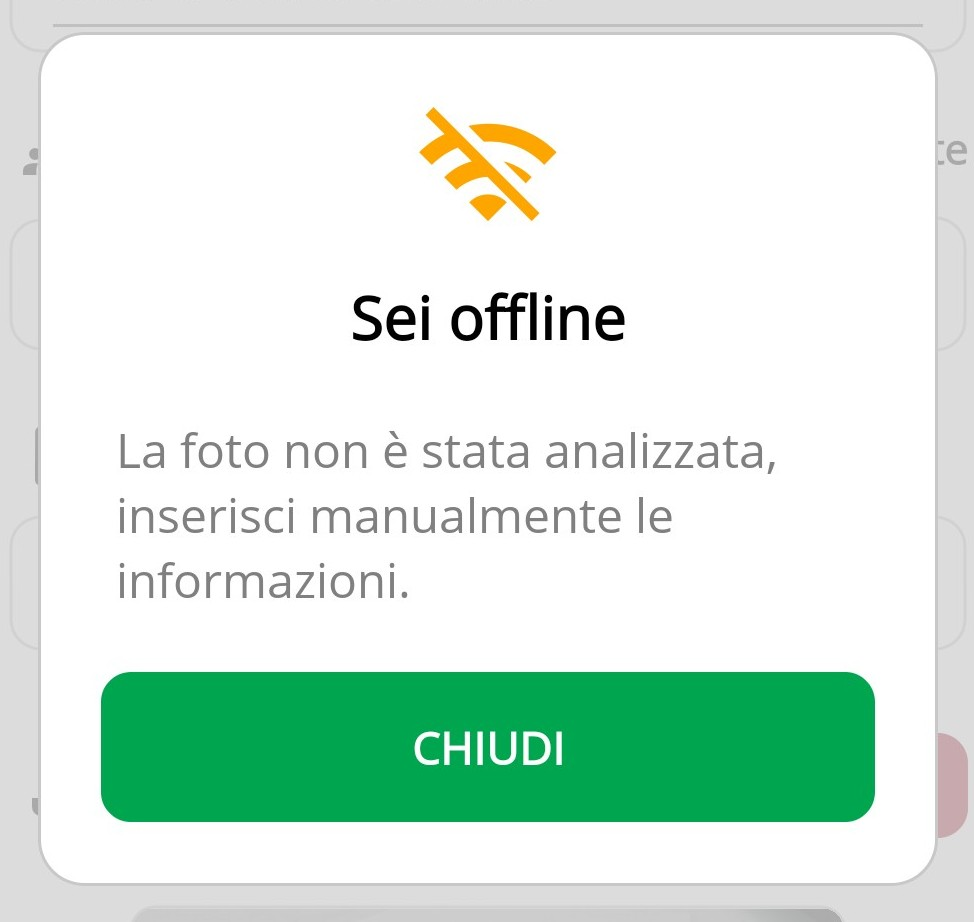
\includegraphics[width=0.29\textwidth]{img/screen/pp_offline.jpg} \\
        \small Pop-up eliminazione & \small Pop-up errore & \small Pop-up offline
    \end{tabular}
    \caption{Esempi di utilizzo del componente GenericPopupView}
    \label{fig:popup}
\end{figure}



\section{Realizzazione delle funzionalità principali}
\label{sec:sviluppo-principali}

\subsection*{L'integrazione con il modulo Planning}
\noindent Un aspetto architetturale di rilievo nello sviluppo del modulo delle note spesa è la sua interoperabilità con i processi informativi preesistenti dell'applicativo aziendale, in particolare con il modulo di pianificazione delle attività (\textit{Planning}). Per ottimizzare l'esperienza utente e ridurre al minimo gli errori di inserimento manuale, è stata implementata una logica di auto-compilazione all'interno del \textit{ViewModel}.\\
Ogni qualvolta l'utente seleziona o modifica la data di competenza di una nuova spesa, il sistema interroga il database locale, ricercando all'interno della tabella \texttt{Planning} l'eventuale presenza di trasferte o appuntamenti assegnati al dipendente per la giornata selezionata. Qualora venga individuata una corrispondenza, il sistema estrae automaticamente il codice identificativo del cliente (\texttt{cod\_cli}) associato all'attività, interroga la tabella anagrafica clienti per recuperarerne la ragione sociale e precompila il relativo campo dell'interfaccia.\\
Questa integrazione, oltre a velocizzare il flusso di inserimento, dimostra come il nuovo modulo non operi come un compartimento isolato, bensì come un'estensione reattiva e interconnessa all'interno dell'ecosistema mobile di Ergon.



\subsection*{Il flusso di acquisizione ed elaborazione IA}
\noindent L'estrazione automatica dei dati rappresenta un elemento cardine dell'esperienza utente nella creazione di una nota spesa. Per garantire un processo fluido e affidabile, il flusso è stato progettato per essere asincrono e per gestire tutti i casi limite in modo trasparente.\\
L'interazione inizia nella vista \texttt{AddNotaSpesaView}, dove una volta attivato il comando dedicato e dopo aver scattato la fotografia o selezionato il file dalla galleria, l'immagine viene presa in carico dal servizio intermedio specializzato, il \texttt{MediaService}. Questo componente esegue operazioni essenziali di ottimizzazione e normalizzazione dell'immagine, come la riduzione della risoluzione e la correzione dell'orientamento, in modo da ridurre l'occupazione di memoria sul dispositivo e minimizzare l'uso della banda di rete e i tempi di trasferimento durante il successivo caricamento verso il server.\\
Una volta completata la fase di pre-elaborazione, il controllo passa al servizio dedicato \texttt{RestService}, che si occupa della comunicazione con i web services aziendali. L'applicazione effettua una richiesta \textit{HTTP POST} verso l'endpoint specifico nel \texttt{NoteSpesaController}, trasmettendo l'immagine all'interno di un \gls{payloadmultipartg}. Il \textit{backend} riceve il file e agisce da tramite verso il cloud di Microsoft, inoltrando l'immagine alle \gls{api} di \gls{azurecontentunderstandingg}. Il servizio  analizza il layout dello scontrino estraendo i dati in modo semantico. La risposta viene restituita al \textit{backend} e da questo mappata in una \gls{dtog} che viaggia a ritroso fino al \textit{frontend} in formato JSON. Il \textit{ViewModel} riceve i dati estratti e popola i campi visivi del form, permettendo all'utente di verificare ed eventualmente correggere le informazioni estratte prima del salvataggio definitivo della nota spesa.

\subsection*{Il funzionamento offline}
\noindent Il pilastro della continuità operativa dell'applicazione è rappresentato dal meccanismo di persistenza locale, strutturato per gestire l'inserimento e la modifica delle note spesa anche in totale assenza di connettività Internet. \\
Quando l'utente conferma il salvataggio di un form tramite la pressione del pulsante "Salva Nota", l'applicazione esegue una routine di validazione. Se l'invio immediato al server non è possibile a causa della mancanza di segnale, o se l'utente sceglie deliberatamente di posticipare l'operazione, la logica interviene instradando il record verso lo strato di memorizzazione locale gestito dalla classe \texttt{ErgDatabase}. Quest'ultimo sfrutta le funzionalità asincrone della libreria \texttt{sqlite-net-pcl} per interagire con il database embedded \gls{sqliteg} residente nel dispositivo.\\
Durante l'inserimento offline nella tabella SpesaDettaglio, l'applicazione assegna al record un identificativo univoco locale e imposta la proprietà booleana \texttt{IsLocale} al valore vero. Inoltre, il modello conserva sia il percorso fisico dell'immagine dello scontrino all'interno del file system protetto del dispositivo, sia le chiavi esterne relative ai dizionari di decodifica (tipologia di spesa e metodo di pagamento) precedentemente scaricati e storicizzati. Il record viene così congelato in uno stato transitorio sicuro, garantendo che nessuna informazione o file multimediale vada perduto in caso di chiusura forzata dell'applicazione o spegnimento dello smartphone.

\subsection*{L'implementazione dei servizi di rete}
\noindent L'integrazione finale e la storicizzazione definitiva delle note spesa nell'\gls{erp} Ergon avvengono attraverso un'architettura di rete flessibile e sicura. \\
Il canale di comunicazione si attiva non appena il dispositivo rileva la presenza di connettività e l'utente avvia l'operazione di sincronizzazione, sia essa globale (tramite il pop-up di riepilogo) o puntuale (dalla schermata di modifica della singola nota locale). L'algoritmo del frontend interroga il database \gls{sqliteg} per estrarre tutti i record il cui flag \texttt{IsLocale} è impostato a vero. Per ogni nota da sincronizzare, l'applicazione prepara un payload JSON strutturato che incapsula tutte le proprietà di business della transazione.\\
La trasmissione dei dati avviene tramite una richiesta \textit{HTTP POST} diretta al \texttt{NoteSpesaController} aziendale, orchestrata all'interno del client mobile avvalendosi della libreria open source RestSharp (\cite{site:restsharp}). L'utilizzo del metodo POST per il transito dei dati risponde a precisi requisiti di sicurezza e aderenza infrastrutturale: consente di veicolare nel corpo della richiesta sia le informazioni contabili della spesa sia i parametri e le credenziali di autenticazione del dipendente in modo cifrato e protetto tramite protocollo HTTPS. Lato server, il controller riceve il payload, esegue una seconda validazione formale dei dati e delega al contesto di \gls{entityframeworkg}  l'inserimento permanente delle righe sul database relazionale centrale. Se la transazione si conclude con successo, il server risponde al client inviando il codice identificativo definitivo generato dal database centrale. Ricevuta la risposta di successo (codice HTTP 200 OK), il \textit{frontend} aggiorna il record locale memorizzando la chiave remota, modifica il flag \texttt{IsLocale} a falso e rimuove in autonomia gli avvisi grafici di mancata sincronizzazione.



\section{Problematiche e soluzioni adottate}
\label{sec:problematiche-soluzioni}
\noindent Durante la realizzazione del modulo delle note spesa, l'attenzione si è focalizzata sul garantire la massima stabilità del software, l'integrità dei dati e un'esperienza utente fluida. A tal fine, sono state analizzate e risolute tre problematiche principali emerse in fase di implementazione.

\subsection*{Mantenimento della reattività dell'interfaccia}
\noindent Il primo ostacolo tecnico ha riguardato la gestione del \textit{Main Thread}, ovvero il flusso di esecuzione interamente dedicato al rendering della veste grafica e alla risposta agli input dell'utente. L'esecuzione di operazioni computazionalmente onerose, come la compressione e l'ottimizzazione delle immagini, l'attesa del completamento delle chiamate di rete o le interrogazioni al database locale, eseguite direttamente sul thread principale rischiavano di causare congelamenti temporanei dell'interfaccia, deteriorando la fluidità percepita dell'app.\\
La soluzione ha previsto l'adozione del paradigma asincrono di \gls{csharpg}, basato sui costrutti \textit{async} e \textit{await} e sulle funzionalità della \gls{tplg}. Le chiamate di rete gestite dal servizio REST e le elaborazioni dei file multimediali sono state rilocate su thread secondari operanti in background. In questo modo, il thread visivo viene immediatamente liberato, consentendo all'interfaccia grafica di rimanere costantemente ricettiva, animata e fluida durante lo svolgimento delle attività di trasferimento dati.

\subsection*{Risoluzione dei conflitti tra dati estratti e input manuale}
\noindent Una seconda problematica, legata alla logica applicativa e all'esperienza utente, si è manifestata nella gestione delle informazioni restituite dal motore \gls{ocr} di Azure. Nel flusso di compilazione di una nota spesa, l'utente ha la facoltà di inserire manualmente alcuni dati prima ancora di allegare l'immagine dello scontrino. Una sovrascrittura automatica e silenziosa dei campi del form da parte dei dati estratti dall'\gls{ia} avrebbe potuto causare la perdita di modifiche intenzionali inserite dal dipendente, generando anomalie o inserimenti errati.\\
Per ovviare a questo problema, è stata sviluppata una logica di controllo nel \textit{ViewModel} preposto all'inserimento. Al rientro del payload JSON contenente i dati dello scontrino analizzato, il sistema esegue un confronto puntuale tra i valori estratti dall'\gls{ia} e quelli già presenti nei campi compilati dall'utente. Qualora vengano rilevate discrepanze su informazioni quali la data o l'importo, l'applicazione interrompe l'automazione e presenta una finestra modale di avviso. Come mostrato in figura \ref{fig:popupconflitti}, questo pop-up mostra esplicitamente i due valori in conflitto, consentendo all'utente di scegliere consapevolmente quale informazione mantenere ed evitando alterazioni non volute dei campi dati.
\begin{figure}[H]
    \centering
    \begin{tabular}{cc}
        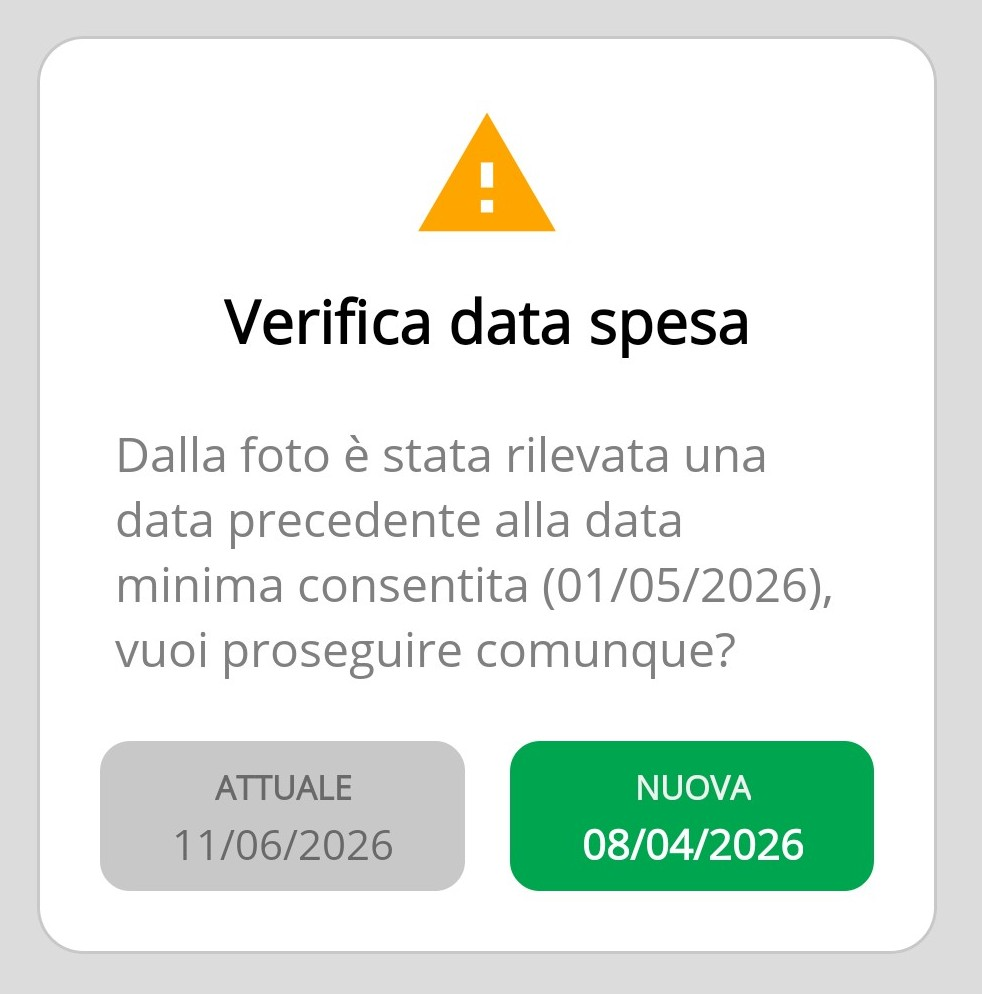
\includegraphics[width=0.29\textwidth]{img/screen/pp_data.jpg} &
        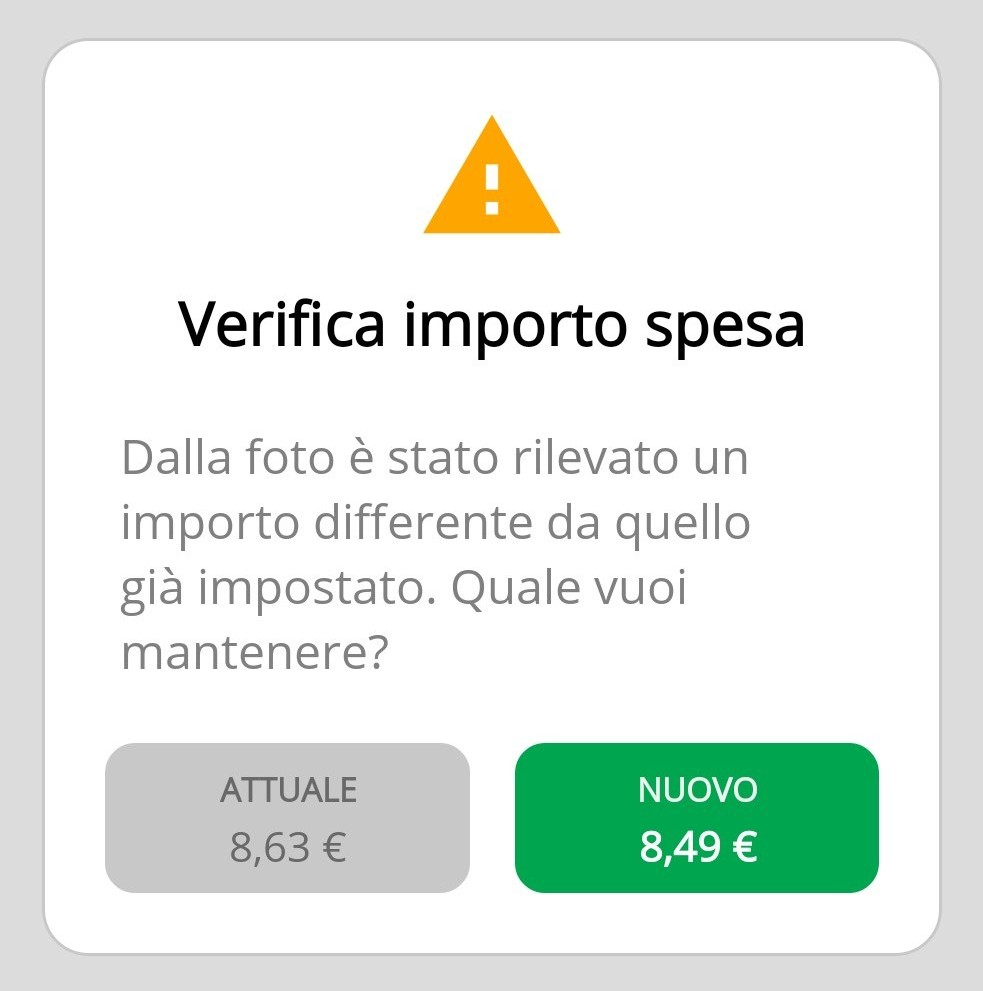
\includegraphics[width=0.29\textwidth]{img/screen/pp_importo.jpg} \\
        \small Pop-up data & \small Pop-up importo
    \end{tabular}
    \caption{GenericPopupView per la gestione dei conflitti}
    \label{fig:popupconflitti}
\end{figure}

\subsection*{Gestione degli accessi concorrenti alle risorse}
\noindent L'ultima sfida ha interessato l'integrità relazionale del database locale. Essendo \gls{sqliteg} basato su un singolo file fisico memorizzato all'interno della memoria protetta dello smartphone, l'esecuzione simultanea di operazioni di lettura e scrittura da parte di flussi diversi può generare eccezioni di blocco del file con conseguenti crash dell'applicazione. Nel contesto dell'applicazione, sebbene l'interfaccia utente sia fortemente protetta da indicatori di caricamento (loader) che inibiscono l'interazione durante le comunicazioni di rete, scenari di concorrenza critici restavano possibili: ad esempio, il lancio simultaneo di due processi asincroni all'avvio dell'applicazione (il controllo delle note locali e il recupero dei dati remoti), oppure un rapido tocco multiplo accidentale da parte dell'utente sul pulsante di salvataggio, in grado di innescare due tentativi di scrittura prima dell'attivazione del blocco visivo.\\
La problematica è stata superata combinando due precise scelte di design. In primo luogo, l'accesso alla risorsa è stato centralizzato a livello di ciclo di vita dell'applicazione tramite una proprietà statica globale all'interno della classe principale \texttt{App}, la quale implementa un meccanismo di inizializzazione per garantire l'esistenza di un'unica istanza condivisa della classe \texttt{ErgDatabase}. In secondo luogo, la sicurezza dei thread sulla connessione \gls{sqliteconnectiong} è stata blindata attraverso l'utilizzo di un oggetto di blocco statico dedicato e del costrutto lock di \gls{csharpg}. Questa istruzione agisce come una barriera di mutua esclusione: quando un thread avvia una transazione, un inserimento o una query, acquisisce l'esclusiva sul blocco, obbligando temporaneamente ogni altra richiesta concorrente ad accodarsi. Al termine dell'operazione, il blocco viene rilasciato in sicurezza, permettendo al processo successivo di accedere al file senza generare conflitti hardware o corruzione dei dati. \\
Di seguito viene riportato un frammento di codice, nel Codice \ref{listing:b}, della classe \texttt{ErgDatabase}, relativo ai principali metodi di inserimento e aggiornamento dei record. Come si può notare, ogni singola operazione sul database sfrutta il costrutto \texttt{lock} applicato all'oggetto statico \texttt{\_locker}. Questa architettura garantisce l'esecuzione sequenziale delle transazioni, mettendo in coda eventuali richieste simultanee ed evitando collisioni o corruzioni del file fisico del database:
\begin{listing}[H]
\begin{minted}{c}
private static readonly object _locker = new object();

private void CreateTableIfNotExists<T>() where T : class, new()
{
    lock (_locker) { Database.CreateTable<T>(); }
}
\end{minted}
\label{listing:a}
\end{listing}

\begin{listing}[H]
\begin{minted}{c}
public bool Insert<T>(T entity) where T : class, new()
{
    lock (_locker)
    {
        try
        {
            CreateTableIfNotExists<T>();
            Database.Insert(entity);
            return true;
        }
        catch
        {
            return false;
        }
    }
}

public int Update<T>(T item) where T : new()
{
    lock (_locker) { return Database.Update(item); }
}
\end{minted}
\caption{Esempio di gestione della connessione con il costrutto lock}
\label{listing:b}
\end{listing}


\section{Valutazione e debito tecnico}
\label{sec:valutazione-debito}
\noindent L'architettura progettata e il codice implementato hanno permesso di raggiungere con successo tutti gli obiettivi prefissati. L'applicazione risulta stabile, usabile e in grado di gestire in totale sicurezza la comunicazione con i sistemi aziendali e l'intero ciclo di vita delle note spesa, anche in condizioni di scarsa connettività. Tuttavia, come in ogni progetto ingegneristico, in fase di collaudo sono emersi dei limiti intrinseci alla soluzione adottata e sono state identificate delle aree di potenziale miglioramento. Questi aspetti costituiscono il cosiddetto "debito tecnico" del progetto, che potrà essere affrontato nei futuri cicli di sviluppo da parte del team aziendale.

\subsection*{Ottimizzazione della gestione dei file multimediali e caching}
\noindent Attualmente, il sistema salva temporaneamente le fotografie degli scontrini nel file system locale del dispositivo in attesa dell'invio al server. Nel caso in cui l'utente effettui una pulizia approfondita della cache di sistema prima di una corretta sincronizzazione, oppure visualizzi una nota già storicizzata il cui file risiede unicamente sul cloud, il sistema ricorre a un approccio conservativo: l'interfaccia mostra un placeholder visivo che indica che l'immagine è disponibile solo in remoto. Un futuro sviluppo dovrebbe prevedere un meccanismo bidirezionale di caching, capace di scaricare in background l'immagine dal server aziendale qualora questa non sia più presente nel file system locale, garantendo così una consultazione sempre completa del documento direttamente dall'app.

\subsection*{Limiti dell'Intelligenza Artificiale e pre-elaborazione}
\noindent L'integrazione di \gls{azurecontentunderstandingg} ha migliorato drasticamente i tempi di compilazione delle note spesa, ma presenta un'inevitabile dipendenza dalla qualità dell'input hardware. Se l'utente acquisisce una fotografia sfocata o in condizioni di scarsa illuminazione, il servizio cloud può restituire dati parziali o fallire l'estrazione. Attualmente, la correzione di eventuali errori è delegata interamente all'utente tramite l'interfaccia. Una possibile evoluzione del sistema potrebbe introdurre una libreria di \gls{computervisiong} direttamente a bordo del dispositivo per effettuare un controllo preventivo sulla nitidezza e sull'inquadratura dell'immagine: in questo modo si potrebbe impedire a priori l'invio al cloud di scatti qualitativamente insufficienti, riducendo il consumo inutile di banda e l'uso di chiamate \gls{api} a pagamento.

\subsection*{Automazione del testing}
\noindent Per quanto riguarda la validazione del codice, le tempistiche stringenti dello stage e la priorità assegnata allo sviluppo delle funzionalità principali e architetturali non hanno permesso l'implementazione di una suite completa di test automatizzati. Attualmente, l'affidabilità del sistema è stata garantita tramite rigorosi collaudi funzionali manuali e l'utilizzo di software esterni per la validazione degli endpoint di rete. Un margine di miglioramento fondamentale per garantire la robustezza e la manutenibilità futura del codice consisterà nell'integrazione di test automatizzati per validare le logiche dei \textit{ViewModel} e di test dell'interfaccia utente.

\newpage